\section{Metaheur\'istica GRASP}
\subsection{Explicaci\'on}

%Explicar detalladamente el algoritmo implementado. Plantear distintos criterios de parada y de seleccion de la lista de candidatos (RCL) de la heurıstica golosa aleatorizada.

La metaheur\'istica \emph{Greedy Randomized Adaptive Search Procedure} (\textbf{GRASP}), es una mezcla de las dos heur\'isticas previas (vistas en \ref{ej3} y \ref{ej4}). Dicho de manera simple: genera un punto de partida de forma golosa para el algoritmo de b\'usqueda local.\\

La distinci\'on de este algoritmo radica en cómo se construye ``\textit{golosamente}'' la soluci\'on inicial.\\

Como la sigla lo indica, consiste en un algoritmo \textit{Goloso Randomnizado}. Es decir que se escogen candidatos a soluci\'on inicial de una manera golosa ligeramente distinta a la ultilizada en la sección anterior. El método \emph{Greedy} de la sección \ref{ej3} escoge a los nodos que van a pertenecer al conjunto solución, de a uno siempre eligiendo al que tiene mayor grado. En cambio, en este caso por cada paso no se elige al nodo de mayor grado sino que se elige uno al azar entre los que ``mejor grado'' tienen.\\ 

Hablar de ``mejor grado'' nos obliga a dar un criterio  para ello, lo que da pie a la definici\'on de la \emph{Restricted Candidate List} (\textbf{RCL}), que es el conjunto de candidatos elegibles para la soluci\'on base.\\

La \emph{\textbf{solución inicial}} se puede formar de diversas maneras. En todos los casos, se añade de a un nodo al conjunto solución hasta que se forme una solución válida. Tres formas para determinar la elección por nodo son: 

\begin{itemize}

\item Elegir un nodo entre los $alpha\%$ nodos que tengan mayor grado hasta completar una soluci\'on v\'alida.

\item Elegir un nodo entre los $alpha$ nodos que tengan mayor grado hasta completar una soluci\'on v\'alida.

\item Elegir un nodo entre los nodos que cumplan determinada propiedad en un $alpha\%$ hasta completar una soluci\'on v\'alida (como por ej: ``Los nodos que tengan grado, a lo sumo, $alpha\%$ menor que el nodo de mayor grado'').

\end{itemize}

Optamos por implementar las primeras dos opciones para generar una solución inicial. Una vez obtenida bajo el método deseado, se aplica el algoritmo de \emph{b\'usqueda local} explicado en el inciso \ref{ej4} sin modificaciones.\\

Un aspecto tambi\'en diferencial de esta heur\'istica, es que no generamos una \'unica instancia inicial, sino que se toma una determinada cantidad de ellas (acorde al criterio de parada). Se ejecuta el algoritmo para la primer instancia y se guarda la solución como \texttt{\'optima}, luego si en alguna ejecución futura se mejora (se obtiene otra solución con menor cantidad de nodos) se actualiza \texttt{\'optima}.\\

Las \emph{\textbf{vecindades}} utilizadas son las mismas que se utilizaron en la heur\'isitca de b\'usqueda local (\ref{ej4}).\\

El \emph{\textbf{criterio de parada}} que adoptamos fue contabilizar las ejecuciones que no produjeron mejora, de modo que sólo se ejecute una determinada cantidad de repeticiones ``malas''. Es decir, siempre que la ejecución otorgue una solución óptima con menos cantidad de nodos que la existente, se seguirá ejecutando. Pero si las ejecuciones no otorgan mejoras se suman al contador, de modo que al llegar a la cantidad indicada se terminará la ejecución.\\

Otra opci\'on podr\'ia haber sido correr un n\'umero fijo de veces y quedarnos con la mejor soluci\'on encontrada; o tambi\'en si conocieramos alguna cota, acercarnos a esta en un determinado porcentaje; o bien una combinaci\'on de todas.

\newpage
\subsection{Experimentaci\'on}

Para analizar qu\'e combinaci\'on de vecindades de b\'usqueda local y elecci\'on de soluci\'on inicial se acercan a encontrar el \'optimo en distintos escenarios, se experiment\'o con una serie de grafos seg\'un criterios:
\begin{itemize}
	\item Mantener los ejes fijos, variando la cantidad de nodos
	\item Mantener los nodos fijos, variando la cantidad de ejes
	\item Grafos Tablero (an\'alogos a los del ``Se\~nor de los Caballos'')
\end{itemize}

\bigskip

Se opt\'o por ejecutar el algoritmo 30 veces y luego, con los tama\~nos de cada conjunto soluci\'on, sacar un promedio.\\

Es decir, obtener un promedio de la cantidad de nodos que requer\'ia la soluci\'on \'optima en cada ejecuci\'on del algoritmo.\\

Luego, sabiendo cu\'antos son los nodos que pertenecen a la soluci\'on \'optima (ejecutando el algoritmo exacto), divimos y obtuvimos en qu\'e porcentaje la heur\'istica falla en encontrar el \textit{\'optimo verdadero}.\\

Las siguientes tabla muestra los valores obtenidos, las columnas 2, 3 y 4 indican el criterio aplicado al grafo; vecindad 2x1 indica que la vecindad usada fue la de quitar dos nodos y agregar uno, vecindad 3x1 quitar tres y agregar uno; n representa el alfa elegido; n mejores indica que como criterio de b\'usqueda de soluci\'on inicial, se tom\'o uno entre los n mejores seg\'un el criterio greedy establecido, n\% mejores indica seleccionar uno entre los que pertenezcan al n\% de los mejores.\\

La diferencia en las dos tablas radica en el criterio de parada, para la primera, se tom\'o la decisi\'on de no seguir buscando si no se modific\'o el \'optimo luego de 5 iteraciones, para la segunda, si no se lo modific\'o luego de 10.\\

\begin{table}[h!]
	\begin{tabular}[c]{|l|l|l|l|l|}
	\hline & Ejes Fijos & Nodos Fijos & Tableros & Porcentaje de error \\
	\hline Vecindad 2x1 3 mejores & 0.1444444444 & 0.0443696313 & 0 & 6.29380252333333\% \\
	\hline Vecindad 2x1 5 mejores & 0.0873015873 & 0.0878199237 & 0.7916666667 & 32.22627259\% \\
	\hline Vecindad 2x1 7 mejores & 0.1272510823 & 0.0897730705 & 0.8083333333 & 34.17858287\% \\
	\hline Vecindad 2x1 10 mejores & 0.0977272727 & 0.1190627034 & 0.75 & 32.2263325366667\% \\
	\hline Vecindad 2x1 12 mejores & 0.1186147186 & 0.1041559051 & 0.4583333333 & 22.7034652333333\% \\
	\hline Vecindad 3x1 3 mejores & 0.278466811 & 0.151036013 & 0.0833333333 & 17.0945385766667\% \\
	\hline Vecindad 3x1 5 mejores & 0.1813888889 & 0.2439944838 & 0.5416666667 & 32.2350013133333\% \\
	\hline Vecindad 3x1 7 mejores & 0.2068867244 & 0.2352629853 & 0.8083333333 & 41.6827681\% \\
	\hline Vecindad 3x1 10 mejores & 0.2764466089 & 0.2326181999 & 0.8333333333 & 44.7466047366667\% \\
	\hline Vecindad 3x1 12 mejores & 0.258968254 & 0.2521559379 & 0.1666666667 & 22.59302862\% \\
	\hline Vecindad 2x1 10\% & 0.086468254 & 0.0821545316 & 0 & 5.62075952\% \\
	\hline Vecindad 2x1 25\% & 0.1322474747 & 0.0895125969 & 0.4583333333 & 22.6697801633333\% \\
	\hline Vecindad 2x1 50\% & 0.1164862915 & 0.0996809898 & 0.7416666667 & 31.9277982666667\% \\
	\hline Vecindad 2x1 75\% & 0.1488816739 & 0.1212623738 & 1.075 & 44.8381349233333\% \\
	\hline Vecindad 2x1 100\% & 0.0852272727 & 0.0990432947 & 1.0333333333 & 40.58679669\% \\
	\hline Vecindad 3x1 10\% & 0.2001839827 & 0.1837163913 & 0 & 12.7966791333333\% \\
	\hline Vecindad 3x1 25\% & 0.1706132756 & 0.1460248135 & 0.1666666667 & 16.1101585266667\% \\
	\hline Vecindad 3x1 50\% & 0.2624531025 & 0.203697747 & 0.4833333333 & 31.64947276\% \\
	\hline Vecindad 3x1 75\% & 0.2133477633 & 0.2416739045 & 0.9416666667 & 46.5562778166667\% \\
	\hline Vecindad 3x1 100\% & 0.2849206349 & 0.2945727019 & 0.4833333333 & 35.42755567\% \\
	\hline
	\end{tabular}
\caption{Promedio de porcentajes de error de GRASP con respecto al algoritmo exacto para cada vecindad y cada selecci\'on de soluci\'on inicial. Con criterio de parada fijado en 5 repeticiones sin mejorar la mejor soluci\'on hallada}
\end{table}
 
\begin{table}[h!]
	\begin{tabular}[c]{|l|l|l|l|l|}
	\hline & Ejes Fijos & Nodos Fijos & Tableros & Porcentaje de error \\
	\hline Vecindad 2x1 3 mejores & 0.1823232323 & 0.0716093318 & 0.3333333333 & 19.5755299133333\% \\
	\hline Vecindad 2x1 5 mejores & 0.1201370851 & 0.0936978155 & 0.4166666667 & 21.01671891\% \\
	\hline Vecindad 2x1 7 mejores & 0.1566738817 & 0.0903101931 & 0.3333333333 & 19.3439136033333\% \\
	\hline Vecindad 2x1 10 mejores & 0.1187950938 & 0.124087402 & 0.6166666667 & 28.65163875\% \\
	\hline Vecindad 2x1 12 mejores & 0.0911976912 & 0.1113699446 & 0.6166666667 & 27.3078100833333\% \\
	\hline Vecindad 3x1 3 mejores & 0.2596572872 & 0.1778930085 & 0.55 & 32.91834319\% \\
	\hline Vecindad 3x1 5 mejores & 0.2637698413 & 0.2698233628 & 0.6333333333 & 38.8975512466667\% \\
	\hline Vecindad 3x1 7 mejores & 0.3213239538 & 0.2286797787 & 0.55 & 36.6667910833333\% \\
	\hline Vecindad 3x1 10 mejores & 0.2844047619 & 0.2735979587 & 0.4833333333 & 34.7112017966667\% \\
	\hline Vecindad 3x1 12 mejores & 0.2242460317 & 0.269319628 & 0.2833333333 & 25.8966331\% \\
	\hline Vecindad 2x1 10\% & 0.0830808081 & 0.0538074353 & 0 & 4.56294144666667\% \\
	\hline Vecindad 2x1 25\% & 0.1161616162 & 0.0841469551 & 0 & 6.67695237666667\% \\
	\hline Vecindad 2x1 50\% & 0.218989899 & 0.1268513858 & 0.325 & 22.36137616\% \\
	\hline Vecindad 2x1 75\% & 0.2454076479 & 0.126309841 & 0.3333333333 & 23.5016940733333\% \\
	\hline Vecindad 2x1 100\% & 0.2024242424 & 0.1329405378 & 0.8333333333 & 38.9566037833333\% \\
	\hline Vecindad 3x1 10\% & 0.1853138528 & 0.1630435123 & 0 & 11.61191217\% \\
	\hline Vecindad 3x1 25\% & 0.2839177489 & 0.2205421872 & 0.1666666667 & 22.37088676\% \\
	\hline Vecindad 3x1 50\% & 0.2687914863 & 0.212152652 & 0.45 & 31.0314712766667\% \\
	\hline Vecindad 3x1 75\% & 0.3088888889 & 0.1862762984 & 0.5916666667 & 36.2277284666667\% \\
	\hline Vecindad 3x1 100\% & 0.3076803752 & 0.2703141941 & 0.9666666667 & 51.4887078666667\% \\
	\hline
	\end{tabular}
\caption{Promedio de porcentajes de error de GRASP con respecto al algoritmo exacto para cada vecindad y cada selecci\'on de soluci\'on inicial. Con criterio de parada fijado en 10 repeticiones sin mejorar la mejor soluci\'on hallada}
\end{table}

\newpage

Para seleccionar la mejor combinaci\'on de par\'ametros de la heur\'istica, respecto a la soluci\'on encontrada contra la \'optima del algoritmo exacto, tomamos como criterio que se minimice la suma de cada fila, es decir, que para casos donde los grafos incrementan su cantidad de ejes, o bien solo su cantidad de nodos, y tableros de caballos, la diferencia contra la \'optima sea m\'inima.\\

Esto nos lleva a que la combinaci\'on \'optima es: Vecindad 2x1 10\% mejores con 10 iteraciones consecutivas sin ver modificaciones en el \'optimo hallado hasta ese momento. Con un error promedio del 4,5\%.\\

Vale tambi\'en para las ejecuciones con 5 iteraciones sin modificar el \'optimo que la misma configuraci\'on es la de menor error promedio (5,6\%).\\

Adem\'as nos interesa ver que sucede con los tiempos de ejecuci\'on, para ver si existe alguna configuraci\'on que convenga aplicar por esta m\'etrica.\\

Para esto, se tomaron tiempos de los mismas instancias para las que analizamos el porcentaje de acierto del \'optimo.\\

En primer lugar analizamos grafos completos y vac\'ios, esperamos que sus gr\'aficos sean par\'abolas cuadr\'aticas, ya que tienen una \'unica soluci\'on posible en cu\'anto a la cantidad de nodos de la misma. Recordando que GRASP ejecuta una adaptaci\'on del algortimo Greedy de costo $O(n^2)$ y sabiendo que el algoritmo de b\'usqueda local retorna en tiempo constante si la soluci\'on hallada es o bien un nodo (grafo completo), o bien todos los nodos del grafo (grafo vac\'io, todas componentes conexas triviales), podemos argumentar por qu\'e esperamos encontrar esa curva particular.\\

  \begin{figure}[h!]
   \begin{center}
 	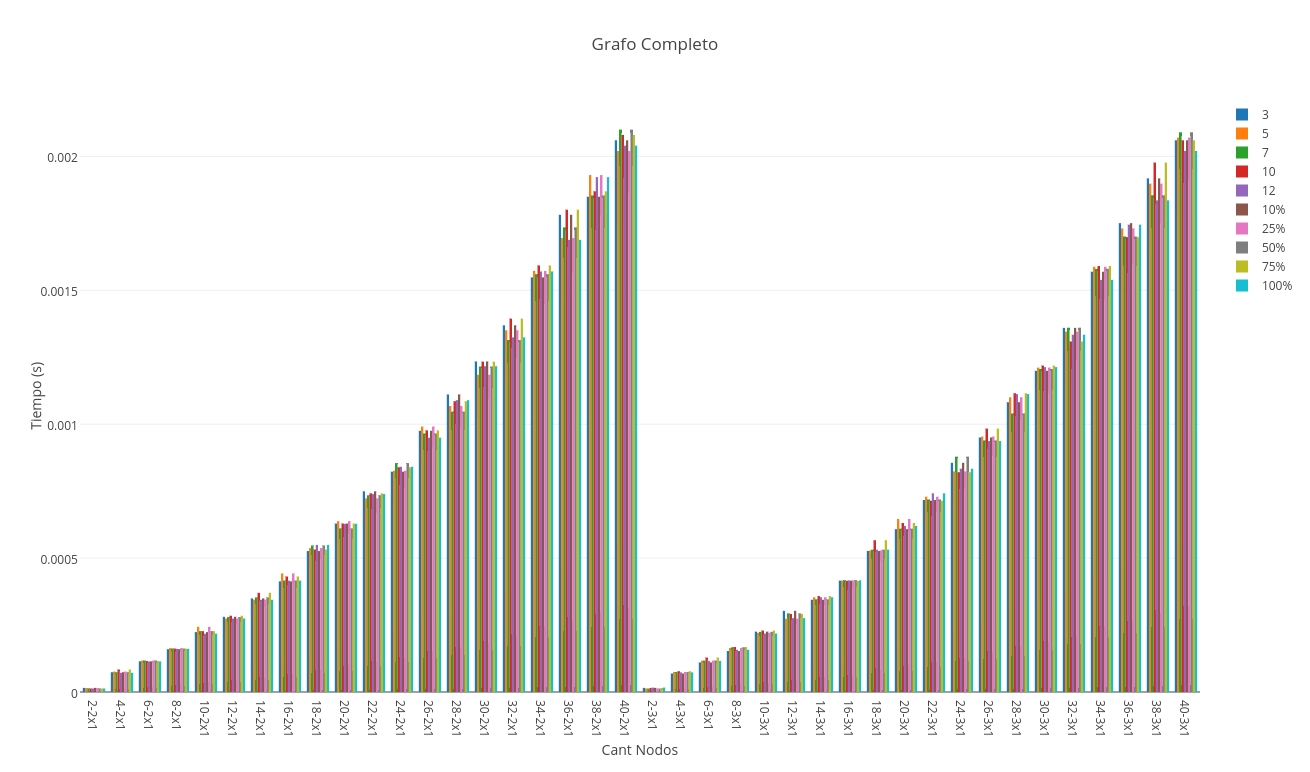
\includegraphics[scale=0.35]{imagenes/grasp/completo-5repes.png}
 	\caption{Comparaci\'on tiempos de ejecuci\'on de la heur\'istica GRASP para grafos completos, aumentando su cantidad de nodos y contrastando las dos vecindades planteadas. Criterio de parada = 5 iteraciones}
	%\label{GrafoCompleto}
   \end{center}
 \end{figure}

  \begin{figure}[h!]
   \begin{center}
 	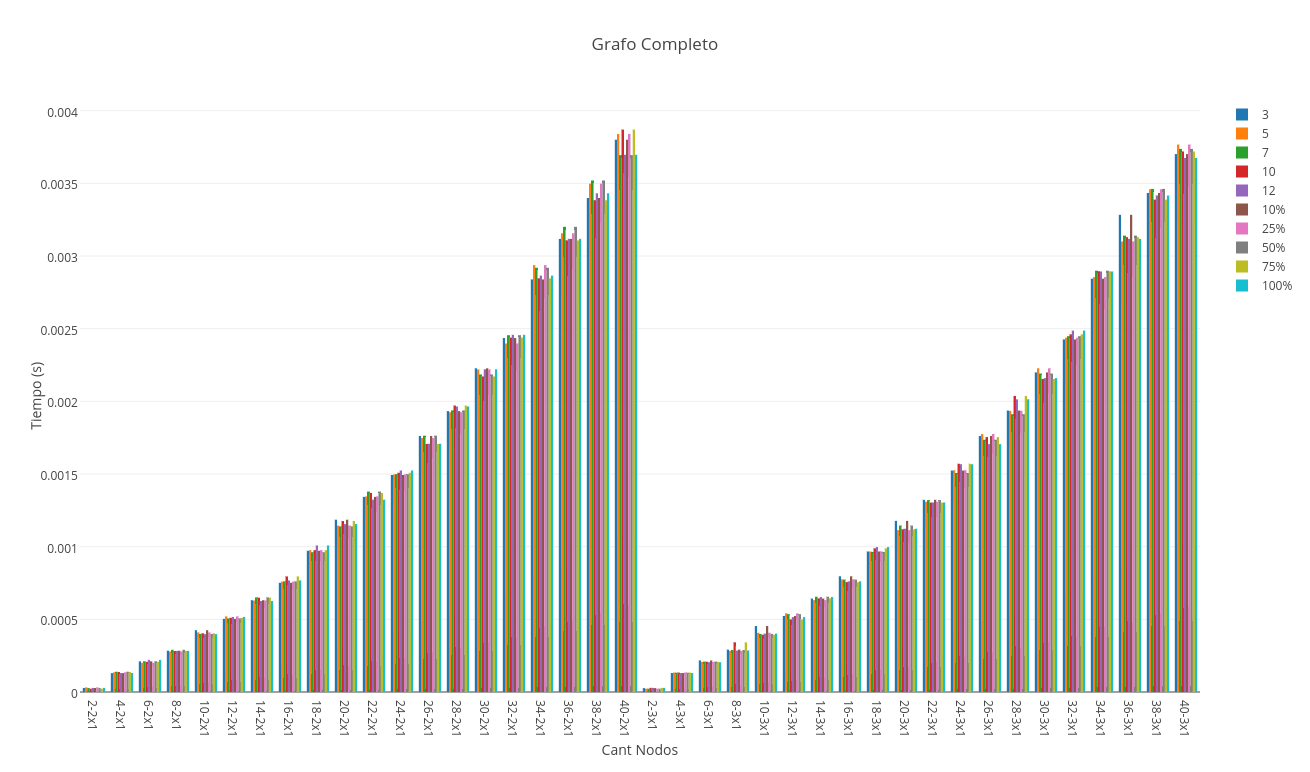
\includegraphics[scale=0.35]{imagenes/grasp/completo-10repes.png}
 	\caption{Comparaci\'on tiempos de ejecuci\'on de la heur\'istica GRASP para grafos completos, aumentando su cantidad de nodos y contrastando las dos vecindades planteadas. Criterio de parada = 10 iteraciones}
	%\label{GrafoCompleto}
   \end{center}
 \end{figure}
\newpage

Estos dos gr\'aficos verifican la curvatura que esper\'abamos para el caso del grafo completo, como tambi\'en que no importa que vecindad se ejecute, pues nunca se intenta mejorar la soluci\'on inicial dado que sabemos que es \'optima por sus caracter\'isticas. Adem\'as se aprecia que el alpha elegido no genera oscilaciones significativas al ejecutarse bajo la misma instancia.

  \begin{figure}[h!]
   \begin{center}
 	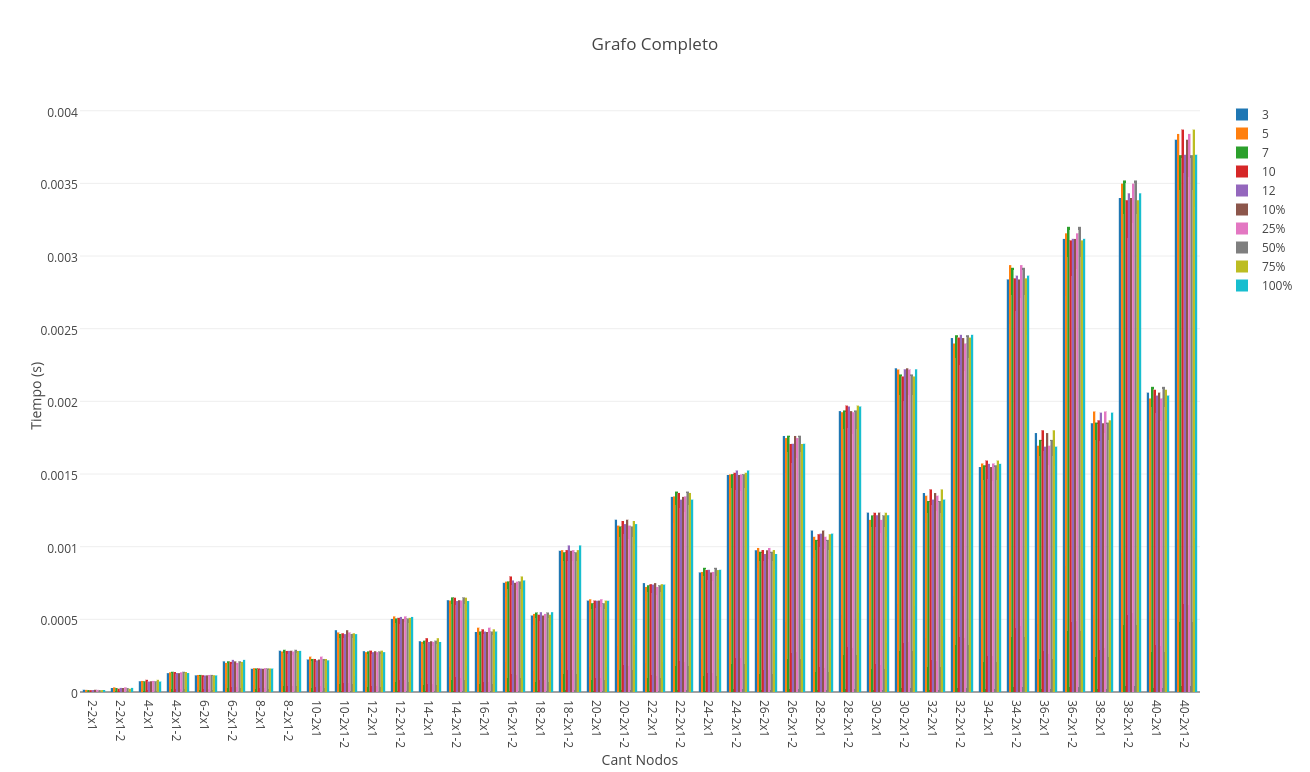
\includegraphics[scale=0.35]{imagenes/grasp/completo-5vs10.png}
 	\caption{Comparaci\'on tiempos de ejecuci\'on contrastando los criterios de parada utilizados}
	%\label{GrafoCompleto}
   \end{center}
 \end{figure}

El anterior permite vislumbrar que efectivamente los criterios de parada afectan al tiempo de ejecuci\'on, se puede ver que las columnas pares duplican a la de su izquierda. Esto se da porque las columnas impares son mediciones sobre no mejorar el \'optimo durante 5 iteraciones y las dem\'as durante 10.

  \begin{figure}[h!]
   \begin{center}
 	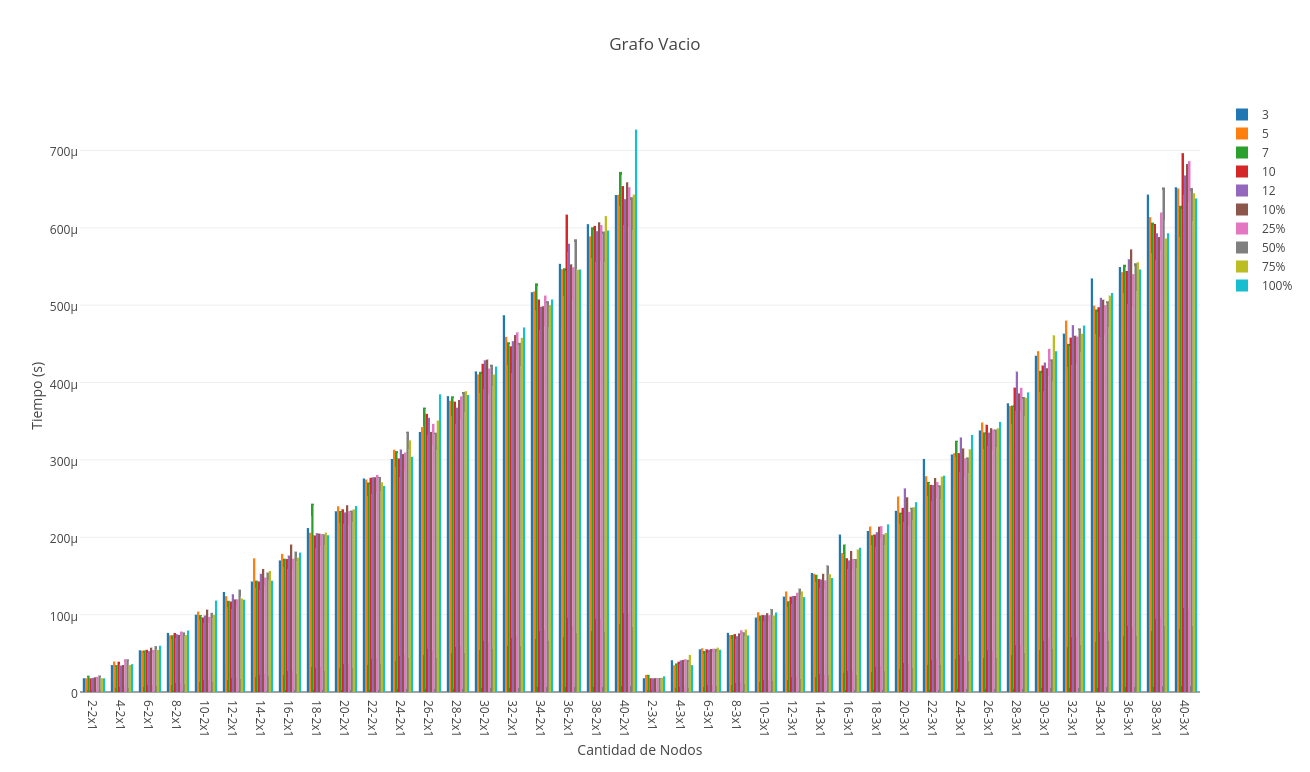
\includegraphics[scale=0.35]{imagenes/grasp/vacio-5repes.png}
 	\caption{Comparaci\'on tiempos de ejecuci\'on de la heur\'istica GRASP para grafos vacios, aumentando su cantidad de nodos y contrastando las dos vecindades planteadas. Criterio de parada = 5 iteraciones}
	%\label{GrafoCompleto}
   \end{center}
 \end{figure}

  \begin{figure}[h!]
   \begin{center}
 	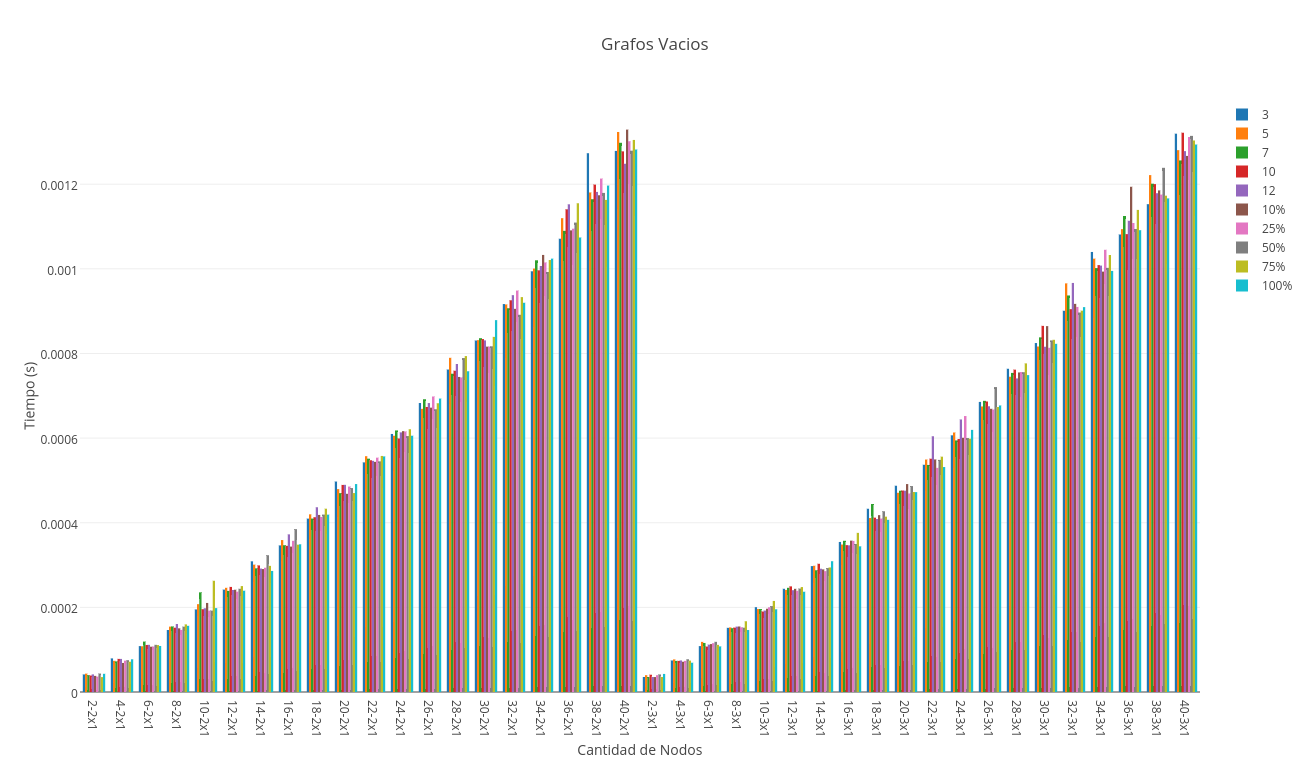
\includegraphics[scale=0.35]{imagenes/grasp/vacio-10repes.png}
 	\caption{Comparaci\'on tiempos de ejecuci\'on de la heur\'istica GRASP para grafos vacios, aumentando su cantidad de nodos y contrastando las dos vecindades planteadas. Criterio de parada = 10 iteraciones}
	%\label{GrafoCompleto}
   \end{center}
 \end{figure}

  \begin{figure}[h!]
   \begin{center}
 	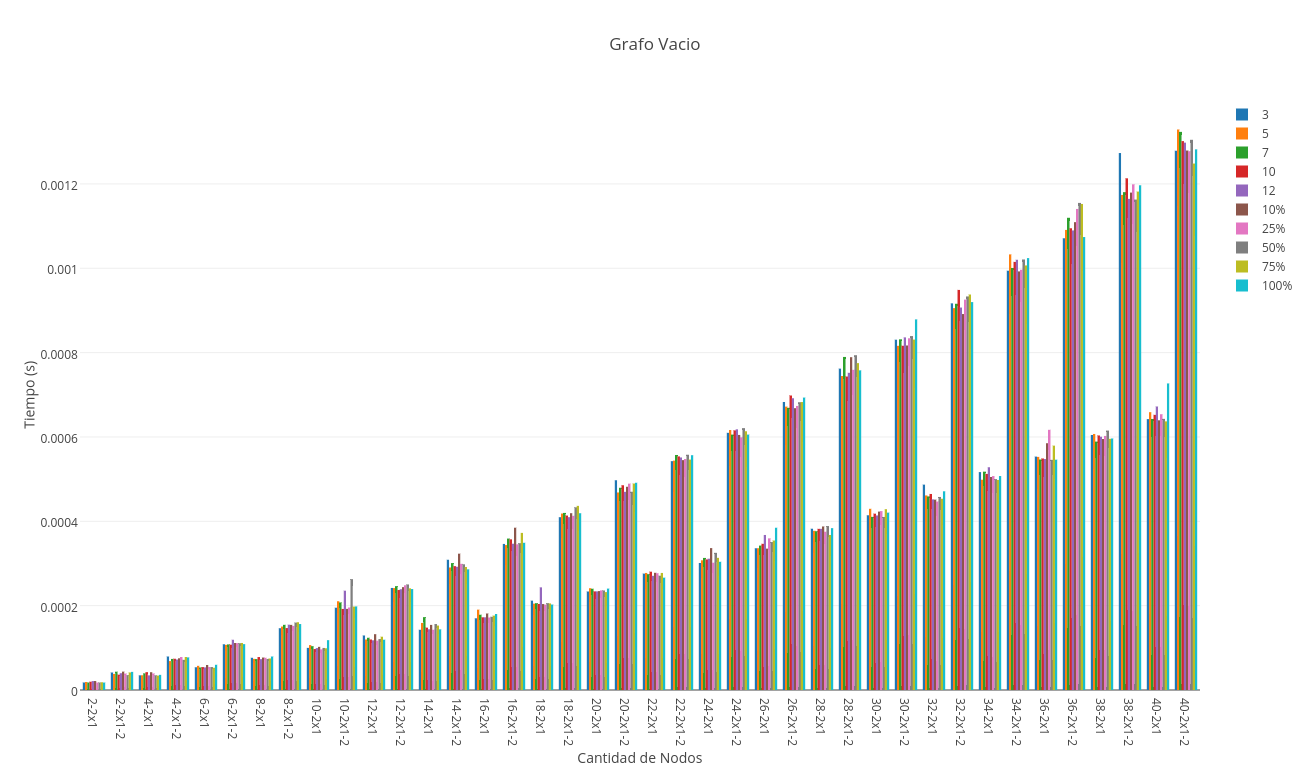
\includegraphics[scale=0.35]{imagenes/grasp/vacio-5vs10.png}
 	\caption{Comparaci\'on tiempos de ejecuci\'on contrastando los criterios de parada utilizados}
	%\label{GrafoCompleto}
   \end{center}
 \end{figure}
\newpage

Estos 3 gr\'aficos de grafos vac\'ios se pueden analizar del mismo modo que a los de grafos completos y verificar que cumplen con las mismas caracter\'iticas, pues son m\'inimas en su conjunto de vecindades asociados.

  \begin{figure}[h!]
   \begin{center}
 	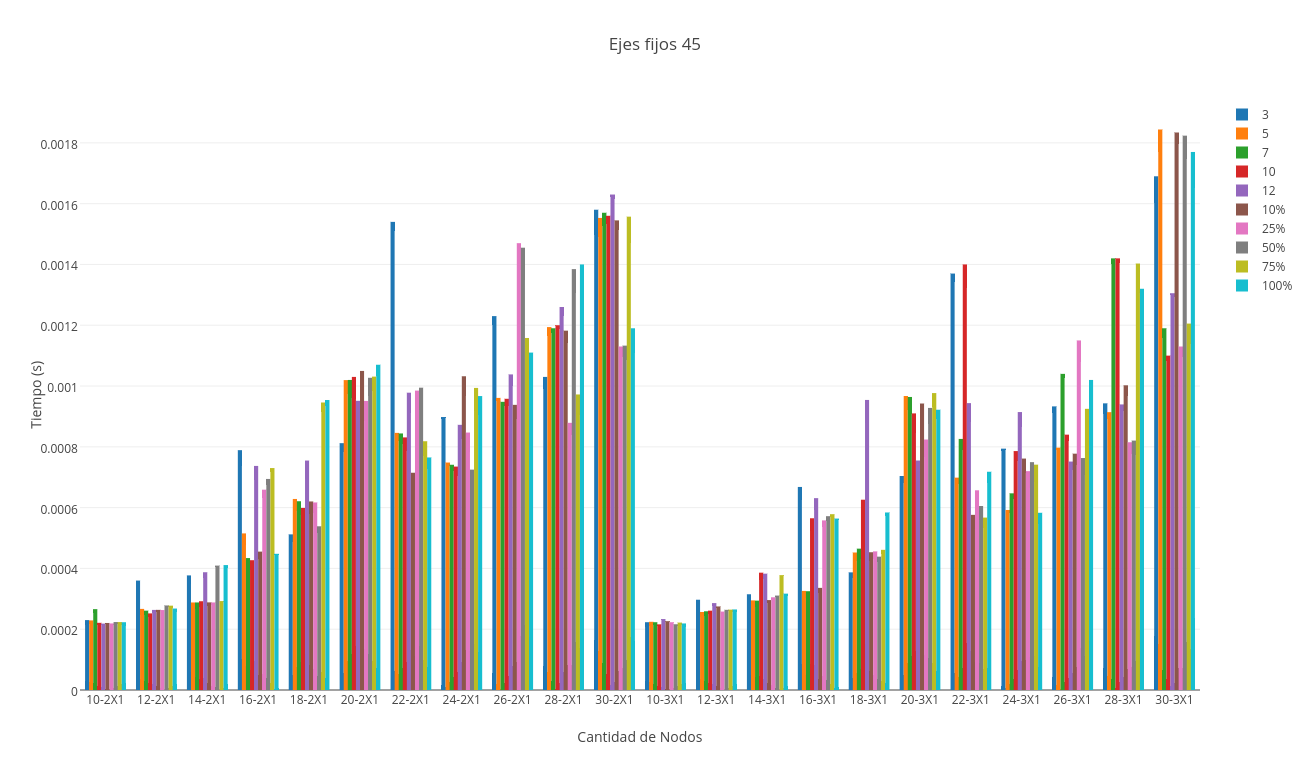
\includegraphics[scale=0.35]{imagenes/grasp/45ejes-5repes.png}
 	\caption{Comparaci\'on tiempos de ejecuci\'on de la heur\'istica GRASP para grafos aleatorios con 45 ejes, aumentando su cantidad de nodos y contrastando las dos vecindades planteadas. Criterio de parada = 5 iteraciones}
	%\label{GrafoCompleto}
   \end{center}
 \end{figure}
\newpage

Este gr\'afico y el siguiente muestran lo analizado en las secciones de las heur\'isticas anteriores, los tiempos de ejecuci\'on dependen de la cantidad de nodos que posea el grafo.\\

Mantener la cantidad de ejes fija y modificar la cantidad de nodos implica que no tendremos una soluci\'on trivial como en los casos anteriores, entonces el algoritmo comienza a revisar la vecindad de la soluci\'on inicial. C\'omo el m\'etodo para generarla es randomnizado, a priori no sabemos cu\'antas veces actualizar\'a su \'optimo, y esto explica los altos y bajos para algunas ejecuciones de la misma instancia para distintos alphas y vecindades; no obstante se observa que se mantiene una marcada relaci\'on instancia-tiempo de ejecuci\'on m\'as all\'a de la vecindad seleccionada.\\

  \begin{figure}[h!]
   \begin{center}
 	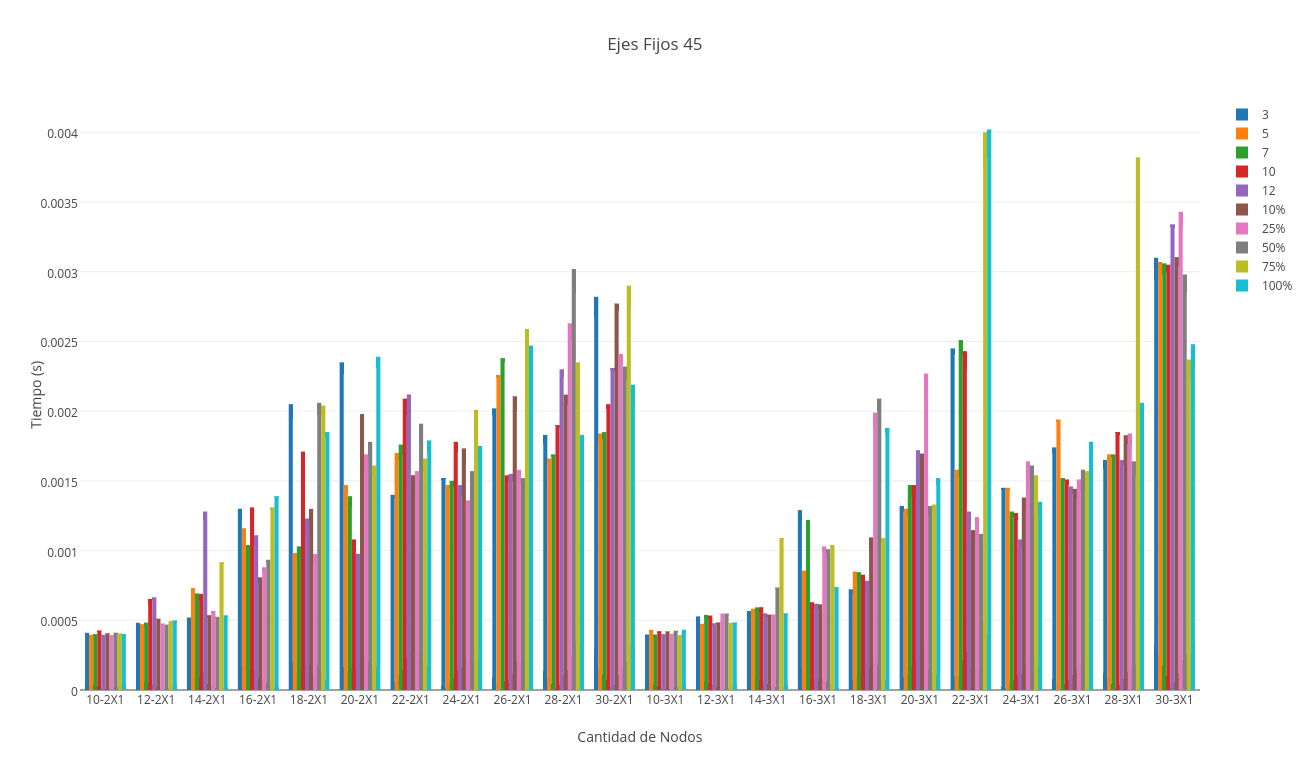
\includegraphics[scale=0.35]{imagenes/grasp/45ejes-10repes.png}
 	\caption{Comparaci\'on tiempos de ejecuci\'on de la heur\'istica GRASP para grafos aleatorios con 45 ejes, aumentando su cantidad de nodos y contrastando las dos vecindades planteadas. Criterio de parada = 10 iteraciones}
	%\label{GrafoCompleto}
   \end{center}
 \end{figure}

  \begin{figure}[h!]
   \begin{center}
 	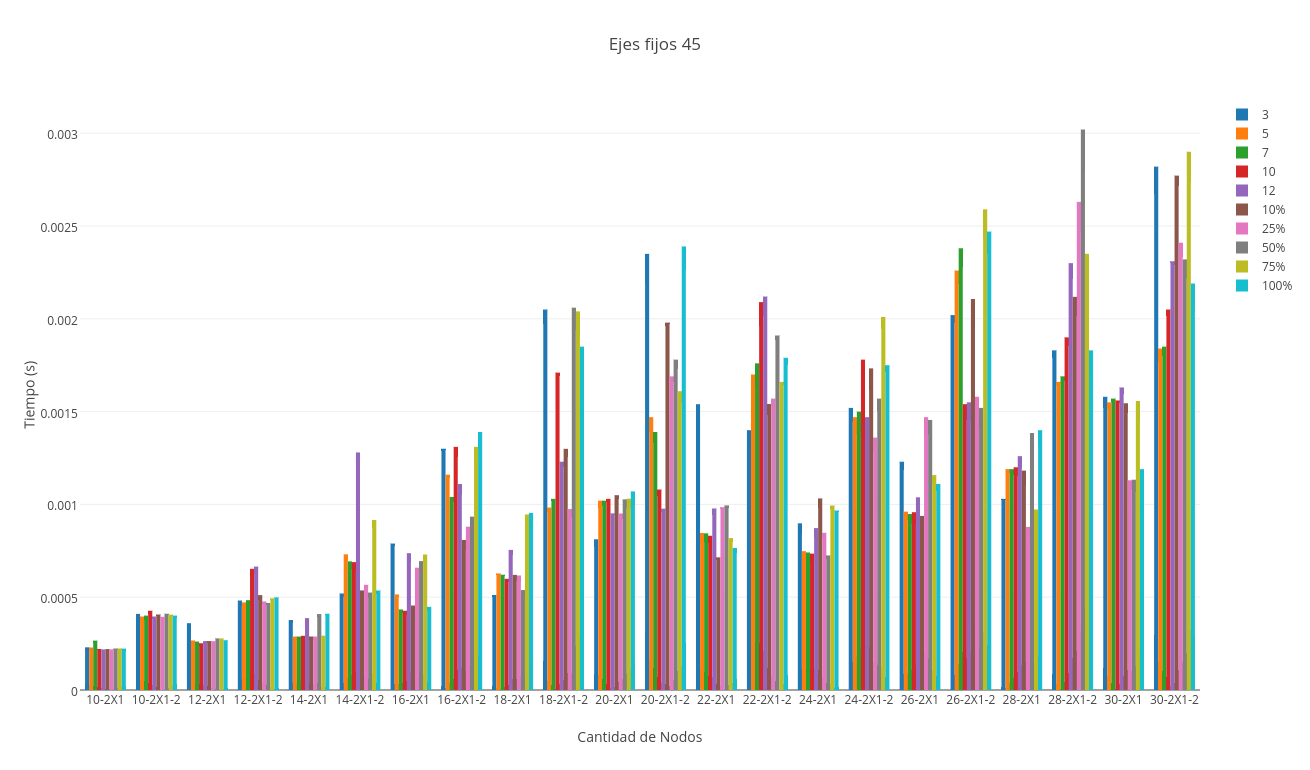
\includegraphics[scale=0.35]{imagenes/grasp/45ejes-5vs10.png}
 	\caption{Comparaci\'on tiempos de ejecuci\'on contrastando los criterios de parada utilizados}
	%\label{GrafoCompleto}
   \end{center}
 \end{figure}
\newpage

Nuevamente, como en los casos Completo y Vac\'io, la tendencia de que parar luego de 10 iteraciones duplique a parar a las 5, se mantiene vigente.

  \begin{figure}[h!]
   \begin{center}
 	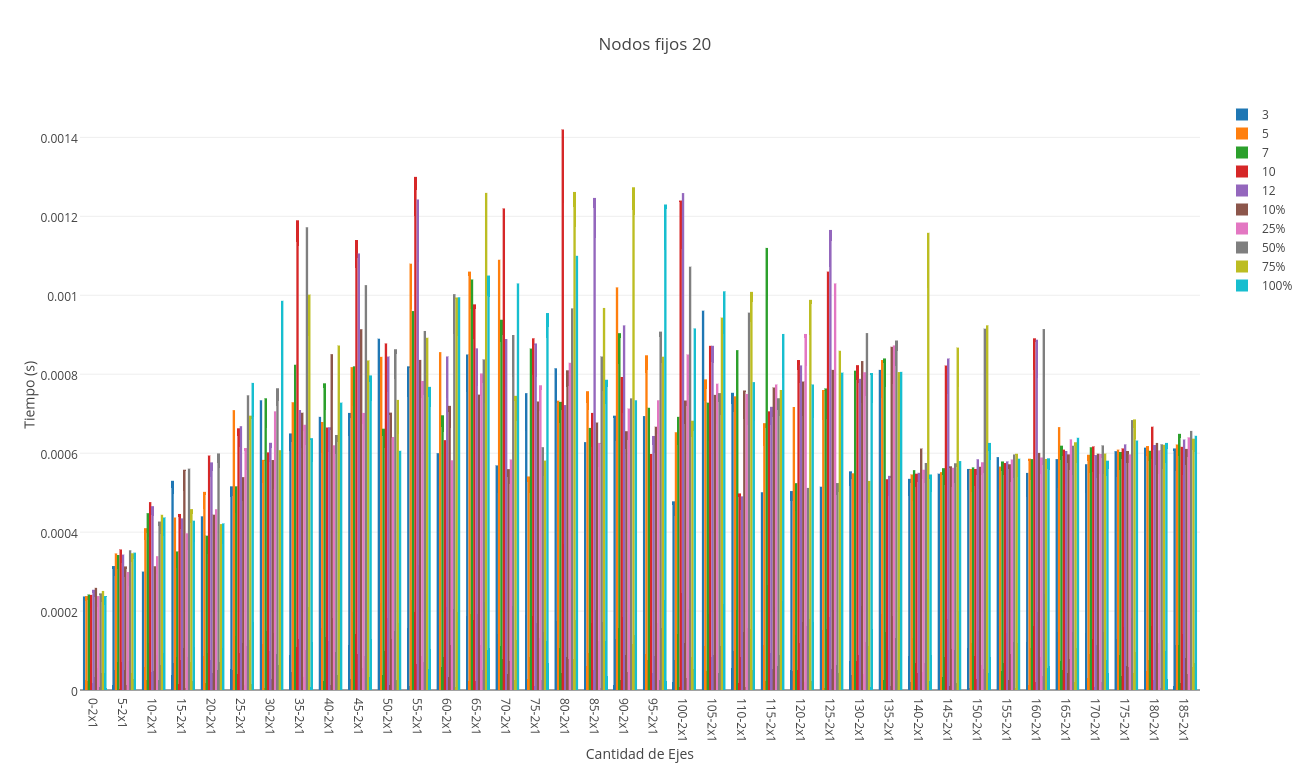
\includegraphics[scale=0.35]{imagenes/grasp/20nodos-5repes-v1.png}
 	\caption{Comparaci\'on tiempos de ejecuci\'on de la heur\'istica GRASP para grafos aleatorios con 20 nodos, aumentando su cantidad de ejes. Criterio de parada = 5 iteraciones. Vecindad 2x1}
	%\label{GrafoCompleto}
   \end{center}
 \end{figure}
\newpage

  \begin{figure}[h!]
   \begin{center}
 	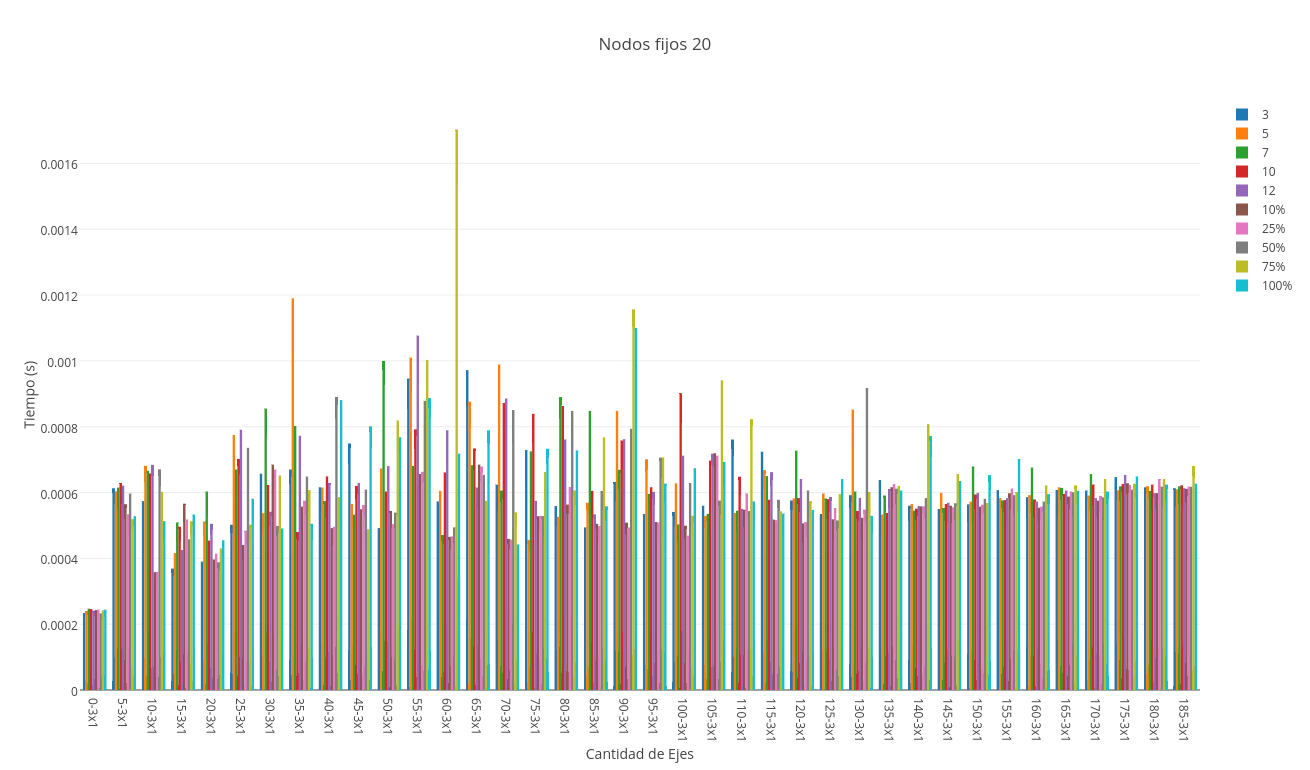
\includegraphics[scale=0.35]{imagenes/grasp/20nodos-5repes-v2.png}
 	\caption{Comparaci\'on tiempos de ejecuci\'on de la heur\'istica GRASP para grafos aleatorios con 20 nodos, aumentando su cantidad de ejes. Criterio de parada = 5 iteraciones. Vecindad 3x1}
	%\label{GrafoCompleto}
   \end{center}
 \end{figure}
\newpage
  \begin{figure}[h!]
   \begin{center}
 	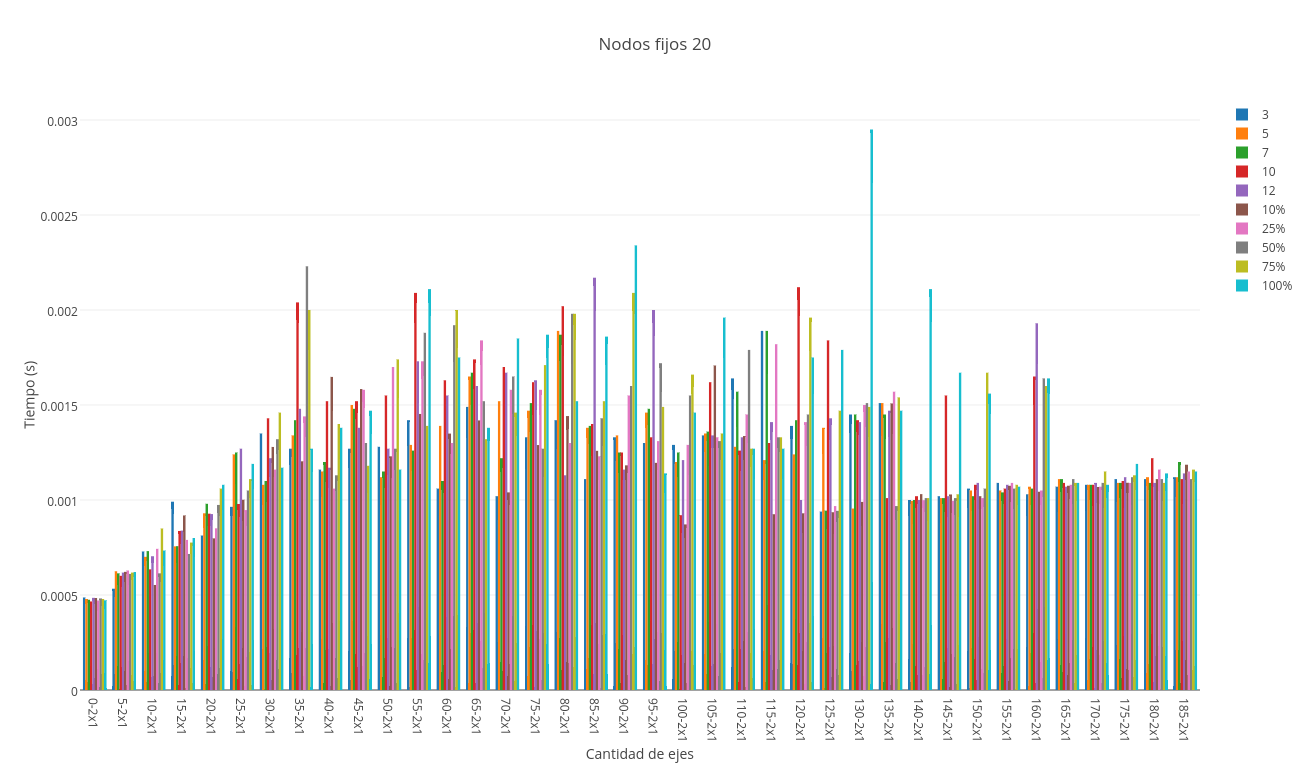
\includegraphics[scale=0.35]{imagenes/grasp/20nodos-10repes-v1.png}
 	\caption{Comparaci\'on tiempos de ejecuci\'on de la heur\'istica GRASP para grafos aleatorios con 20 nodos, aumentando su cantidad de ejes. Criterio de parada = 10 iteraciones. Vecindad 2x1}
	%\label{GrafoCompleto}
   \end{center}
 \end{figure}

  \begin{figure}[h!]
   \begin{center}
 	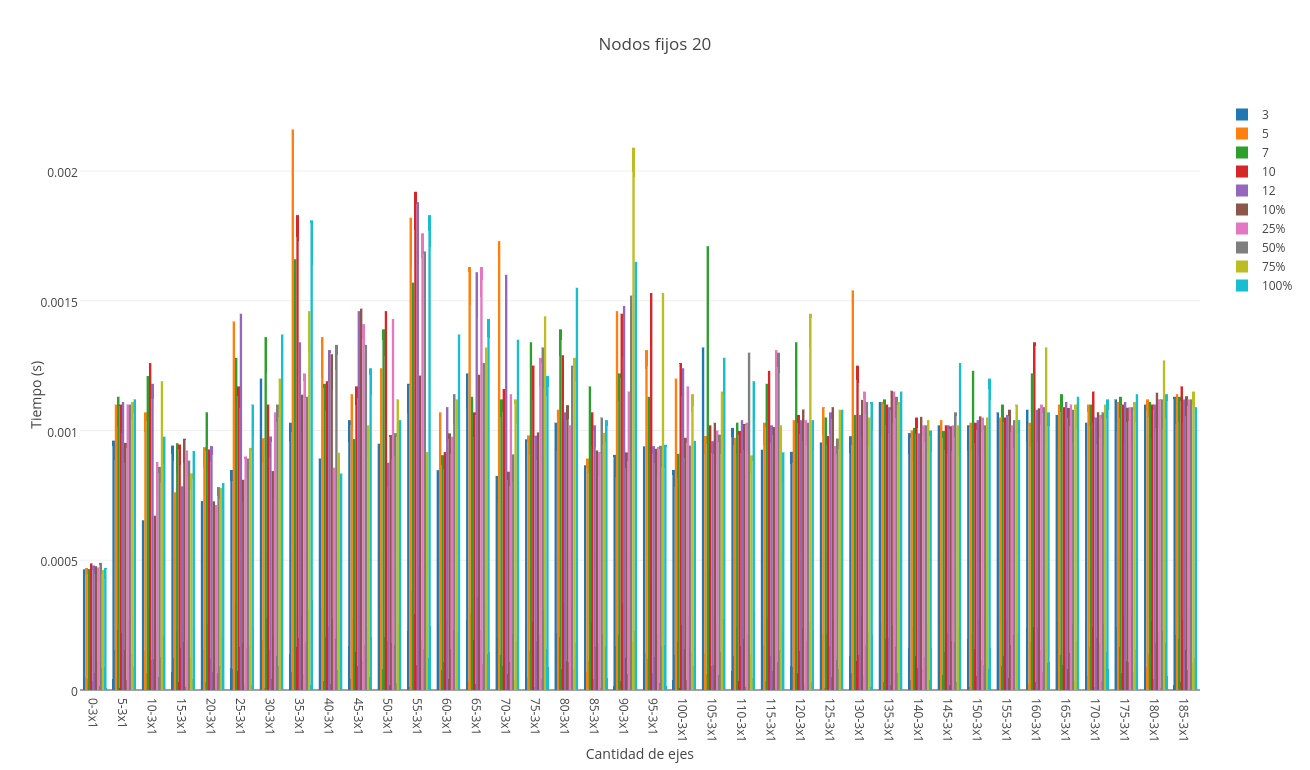
\includegraphics[scale=0.35]{imagenes/grasp/20nodos-10repes-v2.png}
 	\caption{Comparaci\'on tiempos de ejecuci\'on de la heur\'istica GRASP para grafos aleatorios con 20 nodos, aumentando su cantidad de ejes. Criterio de parada = 10 iteraciones. Vecindad 3x1}
	%\label{GrafoCompleto}
   \end{center}
 \end{figure}
\newpage

Estos \'ultimos cuatro gr\'aficos tiene la caracter\'istica de tener un tiempo de ejecuci\'on aproximadamente constante. No obstante en la zona media hay oscilaciones en funci\'on del alpha elegido que no se presentan en los extremos izquierdo y derecho.\\

Esto se debe a que el primer caso es el grafo vac\'io (soluci\'on trivial) y los siguentes poseen muchos ejes aunque no todos, haciendo que la vecindad tarde m\'as en recorrerse completamente.\\

Comparando los tiempos hallados y viendo que las fluctuaciones, entre el alpha elegido y la vecindad tomada no presentan aumentos descomunales en los tiempos de ejecuci\'on, conclu\'imos que salvo para el caso de alpha igual a 100\%, las ejecuciones son de tiempos semejantes.\\

Por lo tanto decidimos que la mejor configuraci\'on para ejecutar la heuer\'istica GRASP es la que mejor resultados provee en cu\'anto a qu\'e tan cerca del \'optimo est\'a. Que como se mencion\'o anteriormente es con alpha = 10\%, y la vecindad 2x1.\\

La distinci\'on entre que itere 5 o 10 veces sin modificar el \'optimo, si bien aqu\'i se concluy\'o que duplica el tiempo de ejecuci\'on, decidimos mantenerlo   en 10 para el experimento del inciso \ref{ej6}. Esto es para poder medir la  diferencia en la soluci\'on hallada por esta heur\'istica en contraposici\'on con la de b\'usqueda local, con una cantidad razonable de instancias iniciales con alta probabilidad de ser distintas entre s\'i.

%Realizar una experimentacion que permita observar los tiempos de ejecucion y la calidad de las soluciones obtenidas. Se debe experimentar variando los valores de los parametros de la metaheurıstica (lista de candidatos, criterios de parada, etc.) y las vecindades utilizadas en la busqueda local. Elegir, si es posible, la configuracion que mejores resultados provea para el grupo de instancias utilizado.
